% Provenance (never printed): cycle 4 SVT, "La planete Terre, l'environnement":
% glaciers and their landforms, the cryosphere, the glaciations told; see
% sources/book1/PROVENANCE.md. Book 1, grade 8, chapter 5.
% Vocabulary guard: owns glacier; ice sheet + ice shelf + iceberg (one
% definition); sea ice; permafrost; U-shaped valley + moraine (one
% definition); ice age. "Glacial period", "interglacial" and "glacial cycle"
% belong to Book 2 g12 past-climates: here "the ice ages and the warmer times
% between them", in prose. Albedo belongs to Book 2 g10: here "reflects".
% Buoyancy and water expanding as it freezes are physics: recalled in prose.
\chapter{La glace sur la Terre}\label{ch:g8:ice-on-earth}

Les deux photographies ci-dessous ont été prises du même endroit, au bord
d'une lagune d'Alaska, à 26 ans d'intervalle. En 1990, une large langue de
glace descendait la \omterm{def:g1:landscapes-around-us:landform}{vallée} jusqu'à l'eau. En 2016, la glace avait reculé
vers le haut de la \omterm{def:g1:landscapes-around-us:landform}{vallée} et s'était rétrécie~; des arbres et de la \omterm{def:g3:stones-pebbles-sand:rock}{roche}
nue occupaient la place qu'elle avait laissée. Entre 1984 et 2021, les
images satellites montrent que le front de ce \omterm{def:g8:ice-on-earth:glacier}{glacier}, le \omterm{def:g8:ice-on-earth:glacier}{glacier}
Pedersen, a reculé d'environ \qty{3.2}{km}.
% ledger: commons:pedersen, uw:pedersen

\begin{omfigure}
\begin{minipage}[t]{0.49\linewidth}\centering
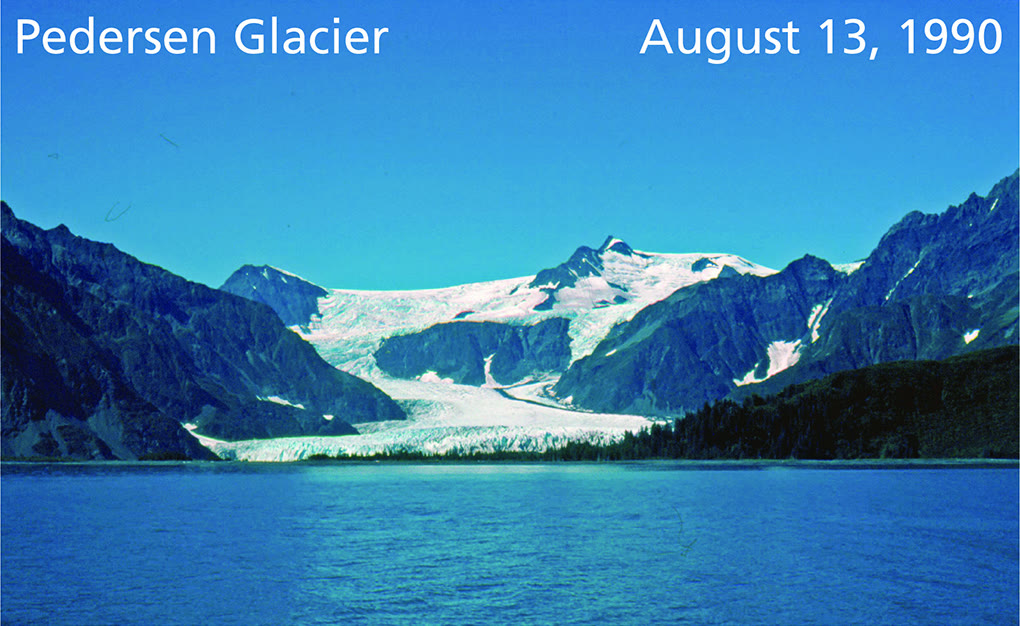
\includegraphics[width=\linewidth]{images/book1/g8-pedersen-1990.jpg}
\end{minipage}\hfill
\begin{minipage}[t]{0.49\linewidth}\centering
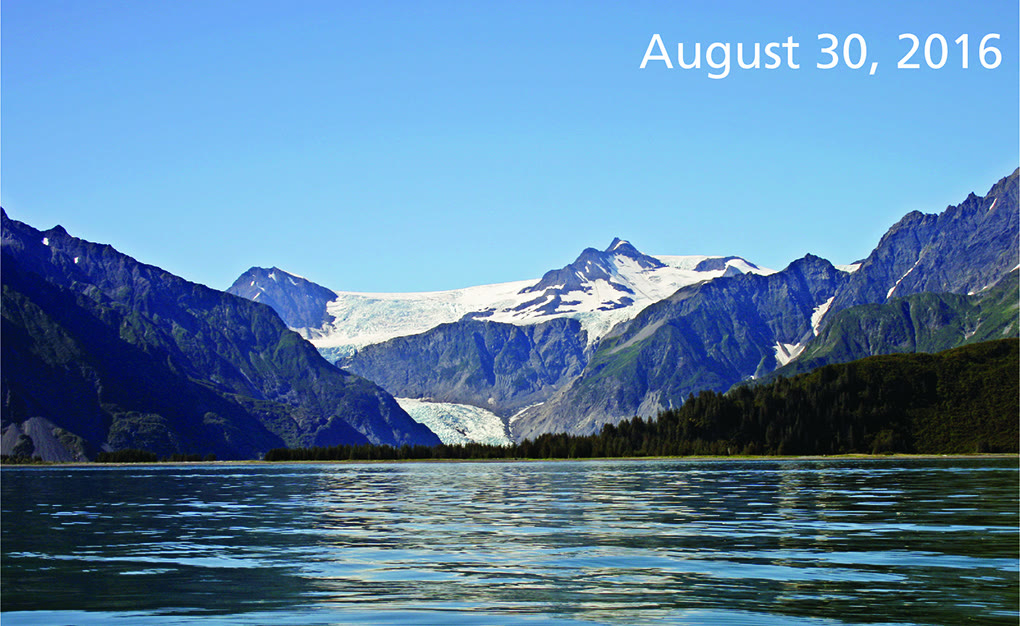
\includegraphics[width=\linewidth]{images/book1/g8-pedersen-2016.jpg}
\end{minipage}

\smallskip
{\small Le \omterm{def:g8:ice-on-earth:glacier}{glacier} Pedersen, parc national de Kenai Fjords, Alaska, vu du
même endroit le 13~août 1990 (à gauche, photographie de M.~Tetreau) et le
30~août 2016 (à droite, photographie de D.~Kurtz). U.S. National Park
Service, domaine public (via Wikimedia Commons).}
% ledger: commons:pedersen
\label{fig:g8:ice-on-earth:pedersen}
\end{omfigure}

La glace couvre aujourd'hui environ un dixième des terres émergées. Elle
occupe des \omterm{def:g1:landscapes-around-us:landform}{vallées} de \omterm{def:g1:landscapes-around-us:landform}{montagne}, deux immenses calottes sur l'Antarctique et
le Groenland, les \omterm{def:g2:water-on-earth:ocean}{mers} polaires et, cachée, l'intérieur du sol gelé du
Grand Nord. Ce chapitre les étudie l'une après l'autre, puis montre comment
la glace façonne le \omterm{def:g4:world-physical-map:relief}{relief}, et revient sur les époques où la glace
couvrait une bien plus grande partie de la Terre qu'aujourd'hui.
% ledger: nsidc:ice-cover

\begin{recall}
La \omterm{def:g4:clouds-rain-snow:precipitation}{neige} est une forme de précipitation~: des cristaux de glace qui
grossissent dans un \omterm{def:g4:clouds-rain-snow:cloud}{nuage} et tombent sans fondre
(\cref{ch:g4:clouds-rain-snow}). L'eau courante érode le \omterm{def:g4:world-physical-map:relief}{relief}, emporte
les débris et les dépose plus loin~; une \omterm{def:g1:landscapes-around-us:water}{rivière} creuse une \omterm{def:g1:landscapes-around-us:landform}{vallée}
(\cref{ch:g5:water-shapes-the-land}). Quand l'eau de \omterm{def:g2:water-on-earth:ocean}{mer} gèle, le sel reste
dans l'eau autour de la glace (\cref{ch:g8:the-oceans}). En physique, on
apprend que l'eau se dilate en gelant, si bien que la glace est moins
dense que l'eau liquide, et qu'un corps plus léger que l'eau qu'il déplace
flotte.
\end{recall}

\section{Les glaciers}

Haut dans les \omterm{def:g1:landscapes-around-us:landform}{montagnes}, il tombe plus de \omterm{def:g4:clouds-rain-snow:precipitation}{neige} en hiver qu'il n'en fond
en été. Année après année, la \omterm{def:g4:clouds-rain-snow:precipitation}{neige} nouvelle recouvre l'ancienne et la
tasse. Les cristaux se serrent, l'air qui les sépare est chassé et, au
bout d'environ un an, la \omterm{def:g4:clouds-rain-snow:precipitation}{neige} est devenue du \emph{névé}, une matière
granuleuse, intermédiaire entre la \omterm{def:g4:clouds-rain-snow:precipitation}{neige} et la glace. Enfoui de plus en
plus profondément, le névé se transforme en glace dure et compacte~; pour
la plupart des \omterm{def:g8:ice-on-earth:glacier}{glaciers}, cela prend plus de cent ans.
% ledger: nsidc:firn

\begin{definition}[Glacier]\label{def:g8:ice-on-earth:glacier}
Un \emph{glacier}\index{glacier} est une masse de glace, formée de \omterm{def:g4:clouds-rain-snow:precipitation}{neige} accumulée pendant
de nombreuses années, qui descend lentement sur le \omterm{def:g4:world-physical-map:relief}{relief} sous son propre
poids.
\end{definition}
% ledger: nsidc:glacier-def

Un \omterm{def:g8:ice-on-earth:glacier}{glacier} a deux parties. Dans sa partie haute, la \emph{zone d'accumulation},
il tombe chaque année plus de \omterm{def:g4:clouds-rain-snow:precipitation}{neige} qu'il n'en fond~: le \omterm{def:g8:ice-on-earth:glacier}{glacier} gagne de
la glace. Dans sa partie basse, la \emph{zone d'ablation}, il fond chaque
année plus de glace qu'il ne tombe de \omterm{def:g4:clouds-rain-snow:precipitation}{neige}~: le \omterm{def:g8:ice-on-earth:glacier}{glacier} perd de la glace.
La glace gagnée en haut descend sans cesse remplacer la glace perdue en
bas. Si les deux s'équilibrent, l'extrémité du \omterm{def:g8:ice-on-earth:glacier}{glacier}, son
\emph{front glaciaire}, reste au même endroit.
% ledger: nsidc:glacier-zones

\begin{omfigure}
\begin{tikzpicture}[font=\footnotesize, >={Stealth[length=2mm]}, xscale=1.08]
  % bedrock
  \fill[black!13] (0,4.6) -- (2,3.9) -- (4,3.0) -- (6,2.0) -- (8,1.1)
    -- (10,0.45) -- (11,0.3) -- (13,0.15) -- (13,-0.5) -- (0,-0.5) -- cycle;
  % the ice body, two zones
  \begin{scope}
    \clip (0,5.5) -- (2,4.9) -- (4,4.0) -- (6,2.9) -- (8,1.8) -- (9.4,0.95)
      -- (10,0.45) -- (8,1.1) -- (6,2.0) -- (4,3.0) -- (2,3.9) -- (0,4.6) -- cycle;
    \fill[omIce] (0,-1) rectangle (5,6);
    \fill[omSea!85] (5,-1) rectangle (11,6);
  \end{scope}
  \draw[black!60] (0,5.5) -- (2,4.9) -- (4,4.0) -- (6,2.9) -- (8,1.8)
    -- (9.4,0.95) -- (10,0.45);
  \draw[black!70, line width=0.6pt] (0,4.6) -- (2,3.9) -- (4,3.0) -- (6,2.0)
    -- (8,1.1) -- (10,0.45) -- (11,0.3) -- (13,0.15);
  % snowline
  \draw[dashed, black!70] (5,2.5) -- (5,4.15);
  \node[anchor=south] at (5,4.15) {chutes de neige = fonte};
  % snowflakes and melting
  \foreach \x/\y in {0.5/6.1, 1.3/5.8, 2.1/5.5, 2.9/5.1, 3.7/4.8, 0.9/6.6, 1.7/6.3, 2.5/6.0, 3.3/5.6, 4.1/5.2}
    \node[omCold] at (\x,\y) {$\ast$};
  \foreach \x/\y in {6.4/2.8, 7.2/2.35, 8.0/1.9}
    \draw[omWarm, decorate, decoration={snake, amplitude=0.6mm, segment length=2mm}] (\x,\y) -- ++(0,0.6);
  % flow arrows inside the ice
  \draw[->, omDef, line width=0.9pt] (1.0,4.72) -- (2.2,4.30);
  \draw[->, omDef, line width=0.9pt] (3.0,3.95) -- (4.2,3.41);
  \draw[->, omDef, line width=0.9pt] (5.2,2.88) -- (6.4,2.28);
  \draw[->, omDef, line width=0.9pt] (7.2,1.84) -- (8.3,1.35);
  % moraine and meltwater
  \fill[omLithCongl] (10.15,0.42) .. controls (10.5,0.95) and (10.9,0.95) .. (11.2,0.29) -- cycle;
  \draw[omSea!60!black, line width=1.6pt] (10.05,0.38) .. controls (10.6,0.22) and (11.4,0.12) .. (12.9,0.08);
  % labels
  \node[align=center] at (1.9,7.35) {zone d'accumulation~:\\ la neige s'entasse,\\ le glacier gagne de la glace};
  \node[align=center] at (10.0,3.3) {zone d'ablation~:\\ la glace fond,\\ le glacier perd de la glace};
  \node[align=left, anchor=west, omDef] at (4.4,1.3) {la glace s'écoule\\ vers le bas};
  \draw[black!60] (10.0,0.5) -- (9.6,-0.1) node[below] {front glaciaire};
  \draw[black!60] (10.7,0.85) -- (11.3,1.4) node[above] {moraine};
  \node[anchor=north east] at (12.9,0.0) {torrent de fonte};
  \node at (2.2,2.6) {roche en place};
\end{tikzpicture}

{\small Un \omterm{def:g8:ice-on-earth:glacier}{glacier} de \omterm{def:g1:landscapes-around-us:landform}{vallée} vu en coupe longitudinale (un croquis, sans
souci d'échelle). Au-dessus de la ligne en tirets, la \omterm{def:g4:clouds-rain-snow:precipitation}{neige} s'accumule plus
vite qu'elle ne fond~; au-dessous, la glace fond plus vite que la \omterm{def:g4:clouds-rain-snow:precipitation}{neige} ne
tombe. La glace s'écoule d'une partie vers l'autre.}
\label{fig:g8:ice-on-earth:long-section}
\end{omfigure}

Comment de la glace solide peut-elle s'écouler~? Sous le poids de la
glace qui la surmonte, la glace profonde d'un \omterm{def:g8:ice-on-earth:glacier}{glacier} se déforme
lentement, comme une épaisse couche de miel froid qui s'étale. Le \omterm{def:g8:ice-on-earth:glacier}{glacier}
glisse aussi sur la \omterm{def:g3:stones-pebbles-sand:rock}{roche} qui le porte, sur une mince pellicule d'eau ou
sur de la \omterm{def:g3:stones-pebbles-sand:sand}{boue} mouillée. Le bas du \omterm{def:g8:ice-on-earth:glacier}{glacier}, qui frotte contre la \omterm{def:g3:stones-pebbles-sand:rock}{roche},
avance plus lentement que sa surface. La plupart des \omterm{def:g8:ice-on-earth:glacier}{glaciers} avancent
lentement et régulièrement~; quelques-uns connaissent soudain une
\emph{avancée brutale}. En 1986, le \omterm{def:g8:ice-on-earth:glacier}{glacier} Hubbard, en Alaska, a avancé
d'environ \qty{10}{m} par jour, et l'avancée brutale la plus rapide jamais
mesurée, celle du \omterm{def:g8:ice-on-earth:glacier}{glacier} Kutiah, au Pakistan, en 1953, a atteint en
moyenne environ \qty{112}{m} par jour pendant trois mois.
% ledger: nsidc:glacier-flow, nsidc:surges

Quand un \omterm{def:g8:ice-on-earth:glacier}{glacier} perd plus de glace en bas qu'il n'en gagne en haut, son
front remonte la \omterm{def:g1:landscapes-around-us:landform}{vallée}~: le \omterm{def:g8:ice-on-earth:glacier}{glacier} \emph{recule}. Un \omterm{def:g8:ice-on-earth:glacier}{glacier} qui recule
continue de s'écouler vers le bas, comme un tapis roulant~; simplement, il
fond plus vite qu'il n'avance. Le \omterm{def:g8:ice-on-earth:glacier}{glacier} Muir, en Alaska, remplissait
toute sa \omterm{def:g1:landscapes-around-us:landform}{vallée} jusqu'à la \omterm{def:g2:water-on-earth:ocean}{mer} en 1941. En 2004, son front avait reculé de
\qty{12}{km}, et la surface de la glace s'était abaissée de plus de
\qty{800}{m}.
% ledger: nsidc:glacier-flow, nsidc:muir

\section{Comment la glace façonne une vallée}

Un \omterm{def:g8:ice-on-earth:glacier}{glacier} est un puissant outil d'\omterm{def:g5:water-shapes-the-land:erosion}{érosion}. Sa glace se soude par le gel à
des blocs de \omterm{def:g3:stones-pebbles-sand:rock}{roche} détachés et les arrache~; les pierres prises dans sa
base raclent la \omterm{def:g3:stones-pebbles-sand:rock}{roche} au-dessous comme du papier de verre. Le \omterm{def:g8:ice-on-earth:glacier}{glacier}
emporte toute cette \omterm{def:g3:stones-pebbles-sand:rock}{roche}, de la fine poussière aux énormes blocs, vers le
bas de la \omterm{def:g1:landscapes-around-us:landform}{vallée} comme un tapis roulant, et la dépose là où la glace fond.
% ledger: nps:u-valley

\begin{omfigure}
\begin{tikzpicture}[font=\footnotesize, >={Stealth[length=2mm]}]
  % V-shaped valley
  \fill[black!13] (0,3) -- (2.1,0.35) -- (2.5,0.35) -- (4.6,3) -- (4.6,-0.4) -- (0,-0.4) -- cycle;
  \draw[black!70, line width=0.6pt] (0,3) -- (2.1,0.35) -- (2.5,0.35) -- (4.6,3);
  \fill[omSea] (2.1,0.35) -- (2.5,0.35) -- (2.42,0.2) -- (2.18,0.2) -- cycle;
  \node[align=center] at (2.3,-0.85) {une rivière creuse une vallée\\ étroite en forme de V};
  % arrow
  \draw[->, line width=1pt] (5.0,1.5) -- (6.2,1.5) node[midway, above, align=center] {un glacier\\ la remplit};
  % U-shaped valley
  \begin{scope}[xshift=6.6cm]
    \fill[black!13] (0,3) .. controls (0.6,1.0) and (0.9,0.25) .. (1.6,0.2)
      -- (3.0,0.2) .. controls (3.7,0.25) and (4.0,1.0) .. (4.6,3) -- (4.6,-0.4) -- (0,-0.4) -- cycle;
    \draw[black!70, line width=0.6pt] (0,3) .. controls (0.6,1.0) and (0.9,0.25) .. (1.6,0.2)
      -- (3.0,0.2) .. controls (3.7,0.25) and (4.0,1.0) .. (4.6,3);
    \draw[dashed, black!40] (0,3) -- (2.1,0.35) -- (2.5,0.35) -- (4.6,3);
    \draw[omCold, line width=0.9pt] (0.37,2.2) -- (4.23,2.2);
    \node[omCold, anchor=south, font=\scriptsize] at (2.3,2.2) {surface de la glace, autrefois};
    \fill[omLithCongl] (0.75,0.95) .. controls (0.95,1.2) and (1.1,1.1) .. (1.2,0.6) -- cycle;
    \fill[omLithCongl] (3.85,0.95) .. controls (3.65,1.2) and (3.5,1.1) .. (3.4,0.6) -- cycle;
    \node[align=center] at (2.3,-0.85) {la glace partie~: une large\\ vallée en U aux versants raides};
    \draw[black!60] (3.65,0.95) -- (4.85,0.6) node[right, align=left] {moraine\\ latérale};
    \node[font=\scriptsize, black!55, align=center] at (2.3,1.6) {(ancien V en tirets)};
  \end{scope}
\end{tikzpicture}

{\small La même \omterm{def:g1:landscapes-around-us:landform}{vallée} de \omterm{def:g1:landscapes-around-us:landform}{montagne} en coupe transversale, avant et après
le passage d'un \omterm{def:g8:ice-on-earth:glacier}{glacier} (un croquis). La glace racle l'étroite \omterm{def:g1:landscapes-around-us:landform}{vallée} de
\omterm{def:g1:landscapes-around-us:water}{rivière} et en fait une large auge au fond plat et aux versants raides, et
laisse des bourrelets de débris rocheux le long de ses bords.}
\label{fig:g8:ice-on-earth:v-and-u}
\end{omfigure}

\begin{definition}[Vallée en U et moraine]\label{def:g8:ice-on-earth:glacial-landforms}
Une \emph{vallée en U}\index{vallee en U@vallée en U} est une \omterm{def:g1:landscapes-around-us:landform}{vallée} au fond large et plat et aux versants
raides, creusée par un \omterm{def:g8:ice-on-earth:glacier}{glacier} qui a élargi et approfondi une étroite
\omterm{def:g1:landscapes-around-us:landform}{vallée} de \omterm{def:g1:landscapes-around-us:water}{rivière} en forme de V. Une \emph{moraine}\index{moraine} est un bourrelet de
débris rocheux, de la poussière aux gros blocs, laissé par un \omterm{def:g8:ice-on-earth:glacier}{glacier}~:
une \emph{moraine latérale} le long de son bord, une
\emph{moraine frontale} à son extrémité.
\end{definition}
% ledger: usgs:erratic, nps:u-valley, nps:moraines

Les \omterm{def:g8:ice-on-earth:glacial-landforms}{moraines} sont des indices précieux. Une \omterm{def:g8:ice-on-earth:glacial-landforms}{moraine} frontale située loin
dans une \omterm{def:g1:landscapes-around-us:landform}{vallée}, sans aucune glace à proximité, montre jusqu'où le \omterm{def:g8:ice-on-earth:glacier}{glacier}
s'avançait autrefois~; une \omterm{def:g8:ice-on-earth:glacial-landforms}{moraine} latérale perchée haut sur un versant
montre quelle était l'épaisseur de la glace. Un gros bloc posé seul dans
un champ, fait d'une \omterm{def:g3:stones-pebbles-sand:rock}{roche} que l'on ne trouve nulle part aux alentours, est
un autre indice~: c'est un \emph{bloc erratique}, une \omterm{def:g3:stones-pebbles-sand:rock}{roche} transportée
loin de son lieu d'origine par un \omterm{def:g8:ice-on-earth:glacier}{glacier} et abandonnée quand la glace a
fondu. Les blocs erratiques vont du simple \omterm{def:g3:stones-pebbles-sand:pebble}{galet} à des blocs plus gros
qu'une maison.
% ledger: nps:moraines, usgs:erratic

\begin{inthefield}[Lire une vallée façonnée par la glace]
Lors d'une promenade en \omterm{def:g1:landscapes-around-us:landform}{montagne}, ou sur la photographie d'une \omterm{def:g1:landscapes-around-us:landform}{vallée} de
\omterm{def:g1:landscapes-around-us:landform}{montagne}, observe la forme de la \omterm{def:g1:landscapes-around-us:landform}{vallée} en coupe~: un V étroit, ou un U
large aux parois raides~? Cherche sur le fond de la \omterm{def:g1:landscapes-around-us:landform}{vallée} de longs
bourrelets de pierres et de terre en désordre qui longent ses versants ou
la traversent~: ce sont peut-être des \omterm{def:g8:ice-on-earth:glacial-landforms}{moraines}. Cherche de gros blocs qui
ne ressemblent pas à la \omterm{def:g3:stones-pebbles-sand:rock}{roche} alentour, et des surfaces rocheuses lisses
rayées de longues lignes parallèles. Reste sur les sentiers, tiens-toi
loin du bord des pentes raides et de la glace elle-même, et dessine ce que
tu vois dans ton carnet.
\end{inthefield}

\section{Calottes glaciaires, plates-formes de glace et icebergs}

Les plus grandes masses de glace de la Terre ne se trouvent pas dans les
\omterm{def:g1:landscapes-around-us:landform}{vallées} de \omterm{def:g1:landscapes-around-us:landform}{montagne}~: elles recouvrent des terres entières. La \omterm{def:g8:ice-on-earth:ice-sheet}{calotte
glaciaire} de l'Antarctique s'étend sur près de
\num{14}~millions de~\unit{km^2} et atteint presque \qty{4.9}{km}
d'épaisseur à son point le plus épais. La calotte du Groenland couvre
environ \num{1.7}~million de~\unit{km^2}, les quatre cinquièmes de l'île,
et dépasse \qty{3}{km} d'épaisseur. À elles deux, elles contiennent plus de
99~\% de la glace des terres émergées, et plus des deux tiers de toute
l'\omterm{def:g2:water-on-earth:salt-fresh}{eau douce} de la Terre.
% ledger: nsidc:ice-sheets

\begin{definition}[Calotte glaciaire, plate-forme de glace et iceberg]\label{def:g8:ice-on-earth:ice-sheet}
Une \emph{calotte glaciaire}\index{calotte glaciaire} est une masse de glace qui couvre plus de
\qty{50000}{km^2} de terres, comme un immense dôme qui s'étale vers
l'extérieur dans toutes les directions. Là où la glace qui s'écoule des
terres atteint la \omterm{def:g2:water-on-earth:ocean}{mer} et continue d'avancer en flottant, toujours
attachée à la glace située derrière elle, elle forme une \emph{plate-forme de glace}\index{plate-forme de glace}.
Un \emph{iceberg}\index{iceberg} est un gros bloc de glace, de plus de \qty{5}{m} de
large, qui s'est détaché d'un \omterm{def:g8:ice-on-earth:glacier}{glacier} ou d'une plate-forme de glace et
flotte sur la \omterm{def:g2:water-on-earth:ocean}{mer}.
\end{definition}
% ledger: nsidc:ice-sheets, nsidc:ice-shelves, nsidc:iceberg

\begin{omfigure}
\begin{minipage}[c]{0.5\linewidth}\centering
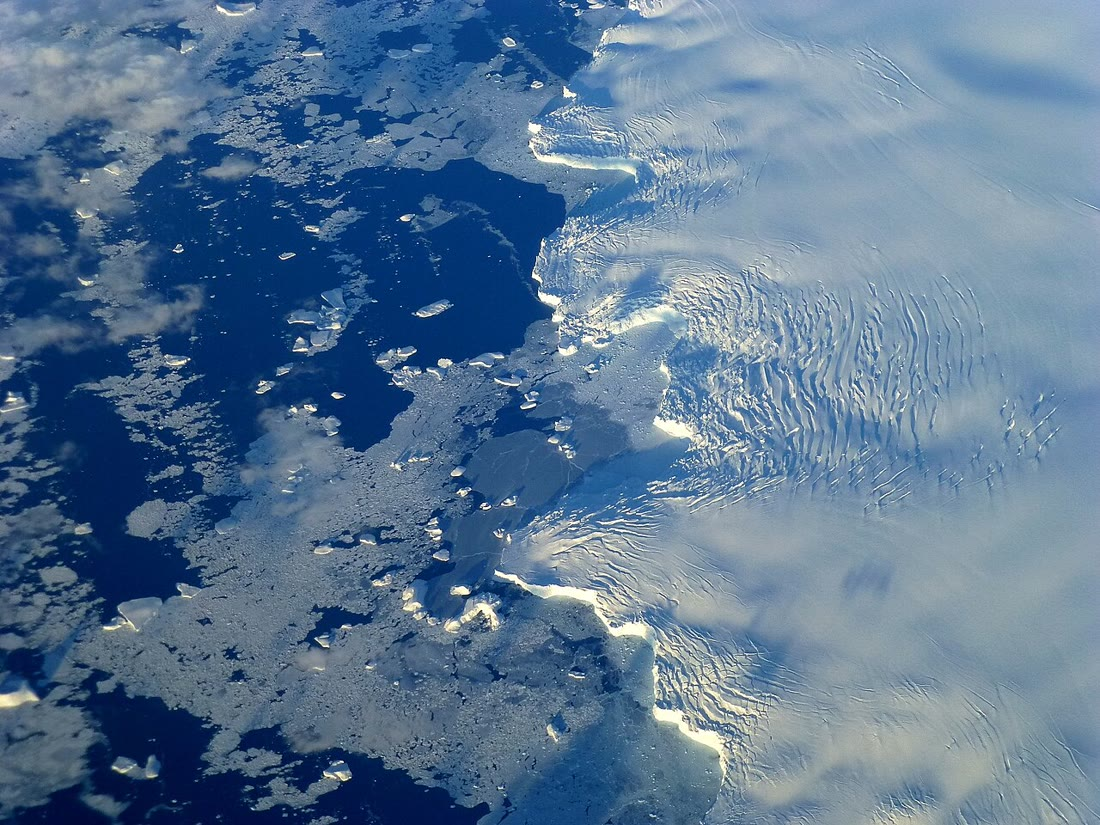
\includegraphics[width=\linewidth]{images/book1/g8-ice-shelf-edge.jpg}
\end{minipage}\hfill
\begin{minipage}[c]{0.46\linewidth}\raggedright
{\small Le bord d'une \omterm{def:g8:ice-on-earth:ice-sheet}{plate-forme de glace} près de l'île Adelaide, au large
de la péninsule Antarctique, vu d'avion le 28~octobre 2012. La glace
épaisse, blanche et plissée, à droite, est la \omterm{def:g8:ice-on-earth:ice-sheet}{plate-forme de glace}~; à
gauche, des morceaux brisés de \omterm{def:g8:ice-on-earth:sea-ice}{banquise} plus mince flottent sur l'eau
sombre. NASA, Operation IceBridge (domaine public, via Wikimedia Commons).}
\end{minipage}
% ledger: commons:ice-shelf
\label{fig:g8:ice-on-earth:ice-shelf}
\end{omfigure}

L'eau prisonnière des \omterm{def:g8:ice-on-earth:ice-sheet}{calottes glaciaires} vient de l'\omterm{def:g2:water-on-earth:ocean}{océan}~: elle s'est
évaporée, est tombée sous forme de \omterm{def:g4:clouds-rain-snow:precipitation}{neige} et s'est accumulée sur les terres.
Si toute la glace du Groenland fondait, la \omterm{def:g2:water-on-earth:ocean}{mer} monterait d'environ
\qty{7.4}{m}~; si toute la glace de l'Antarctique fondait, d'environ
\qty{58}{m}. Tous les \omterm{def:g8:ice-on-earth:glacier}{glaciers} de \omterm{def:g1:landscapes-around-us:landform}{montagne} du monde, plus de
\num{200000}, ajouteraient moins d'un demi-mètre.
% ledger: nsidc:ice-sheets, nsidc:ice-cover

\begin{omfigure}
\begin{tikzpicture}
\begin{axis}[omrecord, xbar, width=10.5cm, height=3.6cm, xmin=0, xmax=68,
  bar width=9pt, ytick=data, symbolic y coords={glaciers,Groenland,Antarctique},
  yticklabels={tous les glaciers de montagne, calotte du Groenland, calotte de l'Antarctique},
  xlabel={hausse du niveau de la mer si tout fondait (m)}, enlarge y limits=0.3,
  nodes near coords, nodes near coords style={font=\footnotesize, anchor=west, fill=white, inner sep=1.5pt},
  ymajorgrids=false]
  \addplot[fill=omIce!80!black, draw=black!60] coordinates {(0.5,glaciers) (7.4,Groenland) (58,Antarctique)};
\end{axis}
\end{tikzpicture}

{\small De combien la \omterm{def:g2:water-on-earth:ocean}{mer} monterait si chaque type de glace terrestre
fondait entièrement (valeurs du National Snow and Ice Data Center~; la
valeur des \omterm{def:g8:ice-on-earth:glacier}{glaciers} est une limite supérieure, «~un peu moins d'un
demi-mètre~»).}
% ledger: nsidc:ice-sheets, nsidc:ice-cover
\label{fig:g8:ice-on-earth:sea-level-bars}
\end{omfigure}

La glace flottante, c'est différent. Une \omterm{def:g8:ice-on-earth:ice-sheet}{plate-forme de glace} ou un
\omterm{def:g8:ice-on-earth:ice-sheet}{iceberg} flotte déjà sur la \omterm{def:g2:water-on-earth:ocean}{mer}~: il a déjà déplacé son propre poids d'eau.
Quand il se brise ou fond, la \omterm{def:g2:water-on-earth:ocean}{mer} ne monte pas. Mais une \omterm{def:g8:ice-on-earth:ice-sheet}{plate-forme de
glace} retient les \omterm{def:g8:ice-on-earth:glacier}{glaciers} situés derrière elle, comme un bouchon dans une
bouteille~; quand la plate-forme Larsen~B, en Antarctique, s'est disloquée
en 2002, les \omterm{def:g8:ice-on-earth:glacier}{glaciers} qui se trouvaient derrière elle ont accéléré,
certains jusqu'à huit fois leur vitesse d'avant, et ont déversé davantage
de glace terrestre dans la \omterm{def:g2:water-on-earth:ocean}{mer}.
% ledger: nsidc:ice-shelves

\begin{inthelab}[Glace flottante et glace sur les terres]
À l'intérieur, pose un petit caillou dans chacun de deux verres
transparents, de façon qu'il dépasse de l'eau une fois les verres remplis.
Dans le premier verre, fais flotter quelques glaçons sur l'eau. Dans le
second, pose le même nombre de glaçons en équilibre sur le caillou, hors de
l'eau. Remplis les deux verres d'eau jusqu'au même niveau et marque-le au
feutre. Attends que toute la glace ait fondu, puis compare les niveaux
d'eau aux marques. Quel verre se comporte comme la \omterm{def:g2:water-on-earth:ocean}{mer} quand un \omterm{def:g8:ice-on-earth:ice-sheet}{iceberg}
fond, et lequel comme la \omterm{def:g2:water-on-earth:ocean}{mer} quand une \omterm{def:g8:ice-on-earth:ice-sheet}{calotte glaciaire} fond~?
\end{inthelab}

\section{La banquise}

La \omterm{def:g8:ice-on-earth:sea-ice}{banquise} est encore autre chose~: c'est la \omterm{def:g2:water-on-earth:ocean}{mer} elle-même, gelée. Chaque
hiver, la surface des \omterm{def:g2:water-on-earth:ocean}{océans} polaires gèle sur une immense étendue~;
chaque été, une grande partie de cette glace fond de nouveau. Dans
l'Arctique, la glace est au plus bas à la fin de l'été, en septembre, et
au plus haut à la fin de l'hiver, en mars. Depuis la fin des années 1970,
des satellites mesurent chaque jour son \emph{étendue}, la surface de \omterm{def:g2:water-on-earth:ocean}{mer}
dont au moins 15~\% est couverte de glace.
% ledger: nsidc:sea-ice-def

\begin{definition}[Banquise]\label{def:g8:ice-on-earth:sea-ice}
La \emph{banquise}\index{banquise} est de l'eau de \omterm{def:g2:water-on-earth:ocean}{mer} gelée~: elle se forme, s'épaissit et fond
dans l'\omterm{def:g2:water-on-earth:ocean}{océan} lui-même. Elle est différente des \omterm{def:g8:ice-on-earth:ice-sheet}{icebergs} et des plates-formes
de glace, qui flottent sur la \omterm{def:g2:water-on-earth:ocean}{mer} mais sont faits de \omterm{def:g4:clouds-rain-snow:precipitation}{neige} tombée sur les
terres.
\end{definition}
% ledger: nsidc:sea-ice-def

La \omterm{def:g8:ice-on-earth:sea-ice}{banquise} compte bien au-delà des \omterm{def:g3:continents-and-oceans:poles}{pôles}. L'eau de \omterm{def:g2:water-on-earth:ocean}{mer} libre est
sombre~: elle ne réfléchit qu'environ 6~\% de la lumière solaire qu'elle
reçoit et absorbe le reste. La \omterm{def:g8:ice-on-earth:sea-ice}{banquise} en réfléchit de 50 à 70~\%, et la
\omterm{def:g8:ice-on-earth:sea-ice}{banquise} couverte de \omterm{def:g4:clouds-rain-snow:precipitation}{neige} jusqu'à 90~\%. Quand la glace fond, l'eau
sombre qu'elle recouvrait absorbe davantage l'énergie du Soleil et se
réchauffe, ce qui fait fondre encore plus de glace.
% ledger: nsidc:sea-ice-reflect

\begin{omfigure}
\begin{tikzpicture}
\begin{axis}[omrecord, width=13cm, height=5.4cm, xmin=1977, xmax=2027,
  ymin=3, ymax=8.2, xtick={1980,1990,...,2020},
  x tick label style={/pgf/number format/1000 sep={}},
  xlabel={année}, ylabel={étendue (millions de km$^2$)},
  legend style={at={(0.98,0.97)}, anchor=north east, draw=none, fill=white}]
  \addplot[omCold, mark=*, mark size=1.3pt, line width=0.6pt]
    table[x=year, y=extent_Mkm2] {figdata/out/grade-8-sea_ice-extent.dat};
  \addlegendentry{étendue moyenne en septembre}
  \addplot[omWarm, dashed, line width=1pt]
    table[x=year, y=extent_Mkm2] {figdata/out/grade-8-sea_ice-trend.dat};
  \addlegendentry{droite de tendance}
  \node[font=\scriptsize, anchor=north] at (axis cs:2012,3.5) {2012};
\end{axis}
\end{tikzpicture}

{\small L'étendue de la \omterm{def:g8:ice-on-earth:sea-ice}{banquise} arctique chaque mois de septembre,
1979--2025, et la droite qui suit au mieux les points. Données~: NSIDC Sea
Ice Index, version~4 (F.~Fetterer et al., 2025).}
% ledger: data:b1-nsidc-sea-ice (figdata/grade-8/sea_ice.py)
\label{fig:g8:ice-on-earth:sea-ice}
\end{omfigure}

Les points montent et descendent d'une année à l'autre~: le \omterm{def:g1:watching-the-weather:weather}{temps qu'il
fait} chaque été compte. Mais au fil des années, ils baissent nettement.
Pour voir l'évolution derrière ces hauts et ces bas, les scientifiques
tracent une \emph{droite de tendance}, la droite qui passe au plus près
de tous les points.
% ledger: data:b1-nsidc-sea-ice (figdata/grade-8/sea_ice.py)

\begin{method}[Lire une tendance sur un graphique]
\begin{enumerate}
  \item Lis les axes~: ce qui est mesuré, dans quelle unité, sur quelles
        années.
  \item Regarde les points~: y a-t-il une hausse générale, une baisse
        générale, ou ni l'une ni l'autre, derrière les hauts et les bas~?
  \item Lis la droite de tendance à la première et à la dernière année.
  \item Fais la différence, et divise-la par le nombre d'années (ou de
        décennies) qui les séparent~: c'est la variation moyenne par an
        (ou par décennie).
  \item N'accorde pas trop d'importance à une seule année~: un point isolé
        loin de la droite, c'est la \omterm{def:g1:watching-the-weather:weather}{météo}~; la droite, c'est la tendance.
\end{enumerate}
\end{method}

\begin{example}[La banquise de l'Arctique en septembre]
Sur le graphique, la droite de tendance est à environ
\num{7.6}~millions de~\unit{km^2} en 1979 et à environ
\num{4.1}~millions de~\unit{km^2} en 2025. La variation est de $7.6 - 4.1 =
3.5$ millions de~km$^2$ en $2025 - 1979 = 46$ ans, soit 4.6 décennies~:
$3.5 \div 4.6 \approx 0.76$. La \omterm{def:g8:ice-on-earth:sea-ice}{banquise} de septembre a diminué d'environ
\num{0.76}~million de~\unit{km^2} par décennie~: en 46 ans, la droite de
tendance a perdu presque la moitié de sa valeur de 1979. Le point le plus
bas, \num{3.57}~millions de~\unit{km^2} en 2012, se trouve bien au-dessous
de la droite~: cet été-là fut exceptionnel.
\end{example}
% ledger: data:b1-nsidc-sea-ice (figdata/grade-8/sea_ice.py), nsidc:sea-ice-reflect

Les mesures montrent que la \omterm{def:g8:ice-on-earth:sea-ice}{banquise} estivale de l'Arctique est devenue à
la fois moins étendue et plus mince depuis les années 1980, à mesure que
l'Arctique se réchauffait. Le \cref{ch:g9:climate-past-and-present}
examine comment le \omterm{def:g5:weather-and-climate:climate}{climat} de la Terre change, et pourquoi.
% ledger: nsidc:sea-ice-reflect

\section{Le pergélisol}

Dans le Grand Nord, le froid pénètre profondément dans le sol. Sous la
toundra d'Amérique du Nord, du Groenland et du nord de l'Asie, le sol et
la \omterm{def:g3:stones-pebbles-sand:rock}{roche} restent gelés toute l'année, et le sont souvent depuis des
milliers d'années. Seule une mince couche superficielle, la
\emph{couche active}, dégèle chaque été et regèle chaque hiver~; les
plantes y poussent, et l'eau qui ne peut pas s'infiltrer dans le sol gelé
au-dessous forme des mares à la surface.
% ledger: nsidc:permafrost

\begin{definition}[Pergélisol]\label{def:g8:ice-on-earth:permafrost}
Le \emph{pergélisol}\index{pergelisol@pergélisol} est un sol, terre ou \omterm{def:g3:stones-pebbles-sand:rock}{roche}, qui reste à
\qty{0}{\degreeCelsius} ou au-dessous pendant au moins deux années de suite.
\end{definition}
% ledger: nsidc:permafrost

Le \omterm{def:g8:ice-on-earth:permafrost}{pergélisol} s'étend sous environ \num{23}~millions de~\unit{km^2}, un
quart des terres de l'\omterm{def:g3:continents-and-oceans:equator}{hémisphère nord}, et sous environ 85~\% de l'Alaska.
Un sol gelé plein de glace est aussi dur que la \omterm{def:g3:stones-pebbles-sand:rock}{roche}~; quand sa glace
fond, le sol se change en \omterm{def:g3:stones-pebbles-sand:sand}{boue} et s'affaisse. Les routes se fissurent,
les bâtiments penchent et les oléoducs peuvent se rompre~: là où il
traverse le \omterm{def:g8:ice-on-earth:permafrost}{pergélisol}, l'oléoduc trans-Alaska court au-dessus du sol sur
\qty{676}{km}. Le dégel du \omterm{def:g8:ice-on-earth:permafrost}{pergélisol} permet aussi aux restes de plantes
gelés depuis des milliers d'années de se décomposer, et de libérer du
dioxyde de carbone et du méthane dans l'air.
% ledger: nsidc:permafrost, nsidc:permafrost-thaw

\begin{omfigure}
\begin{minipage}[c]{0.5\linewidth}\centering
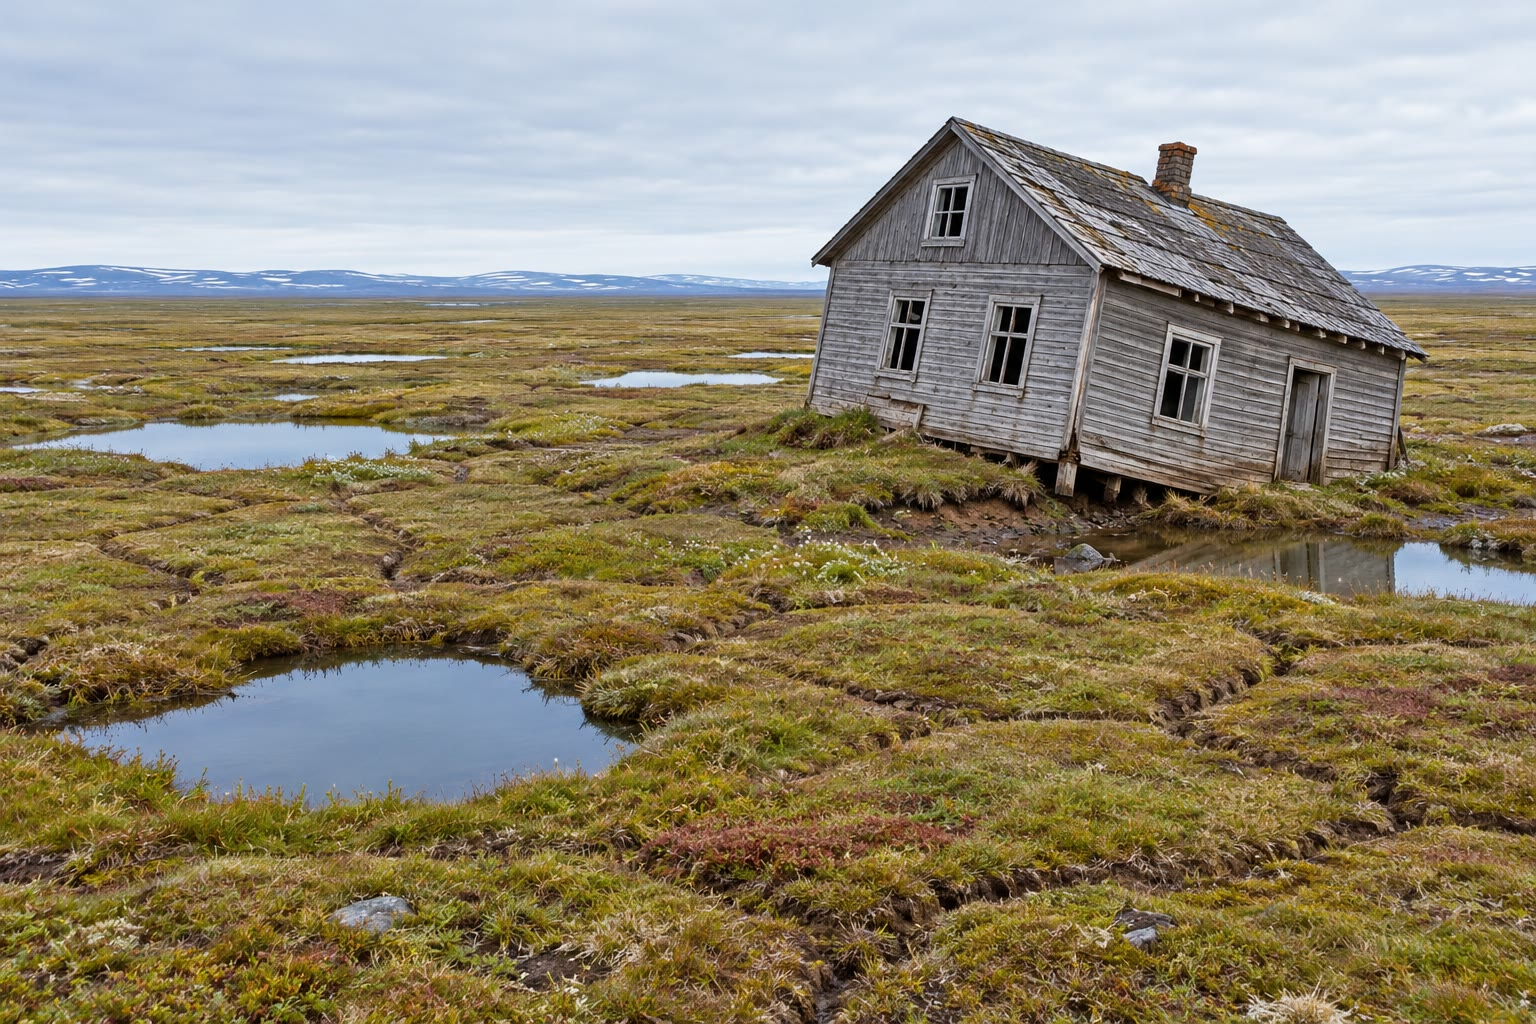
\includegraphics[width=\linewidth]{images/book1/ai/g8-permafrost-house.jpg}
\end{minipage}\hfill
\begin{minipage}[c]{0.46\linewidth}\centering
\begin{tikzpicture}[font=\footnotesize]
  \fill[omLithAlluv] (0,0) rectangle (3.2,-0.6);
  \fill[omIce!70!omLithShale] (0,-0.6) rectangle (3.2,-3.0);
  \foreach \x/\y in {0.4/-1.0, 1.5/-1.3, 2.6/-0.9, 0.9/-1.9, 2.1/-2.2, 0.5/-2.6, 2.8/-2.6}
    \fill[white] (\x,\y) ellipse (0.22 and 0.06);
  \fill[omLithShale!60] (0,-3.0) rectangle (3.2,-3.6);
  \draw[green!45!black, line width=1pt] (0,0) -- (3.2,0);
  \node[anchor=west, align=left] at (3.3,-0.3) {couche active~:\\ dégèle chaque\\ été};
  \node[anchor=west, align=left] at (3.3,-1.8) {pergélisol~:\\ gelé toute\\ l'année,\\ lentilles de glace};
  \node[anchor=west, align=left] at (3.3,-3.3) {sol non\\ gelé};
\end{tikzpicture}
\end{minipage}

\smallskip
{\small À gauche~: une maison qui penche sur un \omterm{def:g8:ice-on-earth:permafrost}{pergélisol} en dégel, dans la
toundra (illustration générée par IA d'une scène générique). À droite~:
le sol sous la toundra (un croquis, sans souci d'échelle).}
\label{fig:g8:ice-on-earth:permafrost}
\end{omfigure}

\section{Les glaciations}

La glace n'a pas toujours couvert la même partie de la Terre. Il y a
environ \num{20000} ans, des \omterm{def:g8:ice-on-earth:ice-sheet}{calottes glaciaires} recouvraient une grande
partie de l'Amérique du Nord et du nord de l'Europe, Scandinavie comprise.
Les \omterm{def:g8:ice-on-earth:glacier}{glaciers} couvraient alors environ un quart des terres, contre environ
un dixième aujourd'hui. Tant d'eau était retenue dans cette glace que la
\omterm{def:g2:water-on-earth:ocean}{mer} se trouvait plus de \qty{120}{m} plus bas qu'aujourd'hui~: une partie
des plateaux continentaux actuels était émergée. À partir d'environ
\num{15000} ans avant nous, les calottes ont fondu et reculé, et la \omterm{def:g2:water-on-earth:ocean}{mer} est
remontée~; elle a atteint à peu près son niveau actuel il y a environ
\num{8000} ans.
% ledger: usgs:lgm, nsidc:ice-sheets, nsidc:ice-cover

\begin{definition}[Glaciation]\label{def:g8:ice-on-earth:ice-age}
Une \emph{glaciation}\index{glaciation} est une longue période froide de l'histoire de la
Terre pendant laquelle les \omterm{def:g8:ice-on-earth:ice-sheet}{calottes glaciaires} s'étendent bien au-delà
des régions polaires et recouvrent de grandes parties des \omterm{def:g3:continents-and-oceans:continent}{continents}. La
dernière glaciation a connu son maximum de froid il y a environ
\num{20000} ans et s'est achevée il y a environ \num{12000} ans.
\end{definition}
% ledger: usgs:lgm, nps:u-valley

Les traces de la dernière \omterm{def:g8:ice-on-earth:ice-age}{glaciation} sont partout dans les terres qu'elle
a recouvertes~: des \omterm{def:g8:ice-on-earth:glacial-landforms}{vallées en U} loin de tout \omterm{def:g8:ice-on-earth:glacier}{glacier} actuel, des \omterm{def:g8:ice-on-earth:glacial-landforms}{moraines}
frontales en travers des \omterm{def:g1:landscapes-around-us:landform}{plaines}, des blocs erratiques posés dans les
champs. Et ce n'était pas la seule. Au cours des dernières centaines de
milliers d'années, les \omterm{def:g8:ice-on-earth:ice-age}{glaciations} et les périodes plus chaudes qui les
séparent se sont succédé encore et encore~; nous vivons dans l'une de ces
périodes chaudes. Le \cref{ch:g9:climate-past-and-present} raconte
comment les scientifiques lisent cette longue histoire dans la glace même
de l'Antarctique.
% ledger: nps:u-valley, nps:moraines, usgs:erratic

\section{Exercices}

\begin{exercise}[$\star$]\label{exo:g8:ice-on-earth:1}
À l'aide de la coupe longitudinale d'un \omterm{def:g8:ice-on-earth:glacier}{glacier} de ce chapitre, nomme~:
(a) la partie du \omterm{def:g8:ice-on-earth:glacier}{glacier} où il gagne de la glace~; (b) la partie où il en
perd~; (c) l'extrémité du \omterm{def:g8:ice-on-earth:glacier}{glacier}~; (d) le bourrelet de débris rocheux à
son extrémité.
\end{exercise}

\begin{exercise}[$\star$]\label{exo:g8:ice-on-earth:2}
% ledger: nsidc:firn, nsidc:glacier-flow, nsidc:sea-ice-def
Vrai ou faux~? Corrige les phrases fausses. (a) Un \omterm{def:g8:ice-on-earth:glacier}{glacier} est fait d'eau
de \omterm{def:g2:water-on-earth:ocean}{mer} gelée. (b) La \omterm{def:g4:clouds-rain-snow:precipitation}{neige} met environ un an à devenir du névé. (c) Quand
un \omterm{def:g8:ice-on-earth:glacier}{glacier} recule, sa glace remonte la pente. (d) La \omterm{def:g8:ice-on-earth:sea-ice}{banquise} de
l'Arctique est au plus bas en septembre.
\end{exercise}

\begin{exercise}[$\star$]\label{exo:g8:ice-on-earth:3}
% ledger: usgs:erratic, nsidc:permafrost
Donne le mot qui correspond à chaque description~: (a) une \omterm{def:g1:landscapes-around-us:landform}{vallée} au fond
large et aux versants raides, creusée par la glace~; (b) un bloc
transporté loin de son lieu d'origine par un \omterm{def:g8:ice-on-earth:glacier}{glacier}~; (c) une plaque de
glace flottante encore attachée à la glace des terres~; (d) un sol qui
reste gelé pendant au moins deux années de suite.
\end{exercise}

\begin{exercise}[$\star$]\label{exo:g8:ice-on-earth:4}
% ledger: nsidc:ice-sheets, nsidc:ice-cover
(a) Quelles sont les deux terres couvertes aujourd'hui par des \omterm{def:g8:ice-on-earth:ice-sheet}{calottes
glaciaires}~? (b) Laquelle des deux ferait le plus monter la \omterm{def:g2:water-on-earth:ocean}{mer} si toute
sa glace fondait, et de combien~? (c) Quelle part des terres émergées est
aujourd'hui couverte de glace~?
\end{exercise}

\begin{exercise}[$\star\star$]\label{exo:g8:ice-on-earth:5}
% ledger: data:b1-nsidc-sea-ice (figdata/grade-8/sea_ice.py)
Utilise le graphique de la \omterm{def:g8:ice-on-earth:sea-ice}{banquise} arctique en septembre. (a) Lis
l'étendue en 1979 et en 2012. (b) De combien de millions de~km$^2$ a-t-elle
diminué entre ces deux années~? (c) Quelle fraction de l'étendue de 1979
avait disparu en 2012~? Arrondis à une fraction simple. (d) Pourquoi
est-il plus fiable de comparer la droite de tendance que deux années
isolées~?
\end{exercise}

\begin{exercise}[$\star\star$]\label{exo:g8:ice-on-earth:6}
% ledger: nsidc:muir, uw:pedersen
Le front du \omterm{def:g8:ice-on-earth:glacier}{glacier} Muir a reculé de \qty{12}{km} entre 1941 et 2004.
(a) Combien d'années cela fait-il~? (b) Quel a été son recul moyen par
an, en mètres~? Arrondis à la dizaine de mètres. (c) Le \omterm{def:g8:ice-on-earth:glacier}{glacier} Pedersen a
reculé de \qty{3.2}{km} entre 1984 et 2021. Quel a été son recul moyen par
an~? (d) Quel \omterm{def:g8:ice-on-earth:glacier}{glacier} a reculé le plus vite~?
\end{exercise}

\begin{exercise}[$\star\star$]\label{exo:g8:ice-on-earth:7}
Explique, en quelques phrases et dans l'ordre, comment la \omterm{def:g4:clouds-rain-snow:precipitation}{neige} tombée
haut sur une \omterm{def:g1:landscapes-around-us:landform}{montagne} devient la glace du front d'un \omterm{def:g8:ice-on-earth:glacier}{glacier}, loin en bas
de la \omterm{def:g1:landscapes-around-us:landform}{vallée}. Utilise les mots \emph{névé}, \emph{zone d'accumulation},
\emph{s'écoule} et \emph{zone d'ablation}.
\end{exercise}

\begin{exercise}[$\star\star$]\label{exo:g8:ice-on-earth:8}
% ledger: nsidc:ice-shelves
Deux verres sont remplis jusqu'au même niveau. Dans le verre A, des
glaçons flottent sur l'eau~; dans le verre B, les mêmes glaçons reposent
sur un caillou, au-dessus de l'eau. (a) Une fois la glace fondue, dans
quel verre le niveau a-t-il monté~? (b) Quel verre est un modèle d'\omterm{def:g8:ice-on-earth:ice-sheet}{iceberg}
qui fond dans la \omterm{def:g2:water-on-earth:ocean}{mer}~? D'une \omterm{def:g8:ice-on-earth:ice-sheet}{calotte glaciaire} qui fond sur les terres~?
(c) Pourquoi la dislocation d'une \omterm{def:g8:ice-on-earth:ice-sheet}{plate-forme de glace} compte-t-elle tout
de même pour le \omterm{def:g4:world-physical-map:altitude}{niveau de la mer}~?
\end{exercise}

\begin{exercise}[$\star\star$]\label{exo:g8:ice-on-earth:9}
Une randonneuse traverse une large \omterm{def:g1:landscapes-around-us:landform}{vallée} au fond plat et aux versants très
raides. Au milieu d'un champ, elle trouve un bloc de granite gros comme une
voiture~; toutes les \omterm{def:g3:stones-pebbles-sand:rock}{roches} de la \omterm{def:g1:landscapes-around-us:landform}{vallée} sont des calcaires. Plus haut, un
long bourrelet de pierres en désordre court le long du versant. (a) Quelle
est la forme de la \omterm{def:g1:landscapes-around-us:landform}{vallée}, et qu'est-ce qui l'a creusée~? (b) Comment le
bloc est-il arrivé là~? Comment l'appelle-t-on~? (c) Qu'est-ce que ce
bourrelet, et que t'apprend sa hauteur sur le versant~?
\end{exercise}

\begin{exercise}[$\star\star$]\label{exo:g8:ice-on-earth:10}
% ledger: nsidc:ice-sheets
La \omterm{def:g8:ice-on-earth:ice-sheet}{calotte glaciaire} de l'Antarctique ferait monter la \omterm{def:g2:water-on-earth:ocean}{mer} d'environ
\qty{58}{m} si elle fondait entièrement, et celle du Groenland d'environ
\qty{7.4}{m}. (a) Qu'ajouterait un dixième de la glace du Groenland~?
(b) Qu'ajouterait un centième de la glace de l'Antarctique~? (c) Combien
de fois plus de glace l'Antarctique contient-il que le Groenland~? Arrondis
à l'unité.
\end{exercise}

\begin{exercise}[$\star\star\star$]\label{exo:g8:ice-on-earth:11}
% ledger: data:b1-nsidc-sea-ice (figdata/grade-8/sea_ice.py: mean_1980s, mean_2010s, trend)
L'étendue moyenne de la \omterm{def:g8:ice-on-earth:sea-ice}{banquise} arctique en septembre était de
\num{7.21}~millions de~\unit{km^2} sur les années 1980--1989 et de
\num{4.65}~millions de~\unit{km^2} sur les années 2010--2019. (a) Un
million vaut $10^6$. Écris les deux valeurs en km$^2$, sans le mot
«~million~». (b) De combien l'étendue moyenne a-t-elle baissé entre ces
deux décennies~? (c) Les deux décennies sont séparées de 30 ans. Quelle
est la baisse par décennie~? Compare-la aux \num{0.76}~million
de~\unit{km^2} par décennie de la droite de tendance. (d) Pourquoi ne
peut-on pas prolonger indéfiniment une droite de tendance dans l'avenir~?
\end{exercise}

\begin{exercise}[$\star\star\star$]\label{exo:g8:ice-on-earth:12}
% ledger: usgs:lgm (the shelf slope is exercise data)
Il y a environ \num{20000} ans, la \omterm{def:g2:water-on-earth:ocean}{mer} se trouvait environ \qty{120}{m}
plus bas qu'aujourd'hui. Au large d'une \omterm{def:g1:landscapes-around-us:water}{côte}, le \omterm{def:g8:the-oceans:seafloor}{plateau continental}
descend en pente très douce, de \qty{1}{m} pour chaque \qty{1}{km} vers le
large (données d'exercice). (a) À quelle distance au large se trouvait
la \omterm{def:g1:landscapes-around-us:water}{côte} à cette époque~? (b) Où était passée l'eau des \qty{120}{m}
manquants~? (c) Explique pourquoi une \omterm{def:g8:ice-on-earth:glacial-landforms}{moraine} frontale trouvée aujourd'hui
dans une \omterm{def:g1:landscapes-around-us:landform}{plaine}, loin de toute \omterm{def:g1:landscapes-around-us:landform}{montagne}, est un indice de cette même
\omterm{def:g8:ice-on-earth:ice-age}{glaciation}.
\end{exercise}

\section{Problème~: le long recul d'un glacier}

\begin{problem}[{Problème du week-end --- le front d'un glacier de montagne
est mesuré tous les dix ans depuis 1960~; on calcule sa vitesse de recul,
et on lit la vallée qu'il laisse derrière lui}]
\label{pb:g8:ice-on-earth:1}
% ledger: nsidc:muir, uw:pedersen, nps:moraines (figdata/grade-8/glacier_retreat.py; Glacier G and its measurements are exercise data)
Tous les dix ans depuis 1960, une équipe mesure la position du front du
\omterm{def:g8:ice-on-earth:glacier}{glacier}~G, un \omterm{def:g8:ice-on-earth:glacier}{glacier} de \omterm{def:g1:landscapes-around-us:landform}{vallée} en \omterm{def:g1:landscapes-around-us:landform}{montagne}. La distance est mesurée vers
l'amont, à partir d'un repère~R peint sur le fond de la \omterm{def:g1:landscapes-around-us:landform}{vallée}, au niveau
du front, en 1960. Un refuge~H se dresse au bord du fond de la \omterm{def:g1:landscapes-around-us:landform}{vallée}, à
\qty{1980}{m} en amont de~R. La \omterm{def:g2:drawing-to-map:map}{carte} montre le front à chaque mesure et
le bourrelet situé juste en aval du front de 1960.

\begin{center}
\begin{tikzpicture}
\begin{axis}[axis equal image, width=12.5cm, xmin=-500, xmax=2600, ymin=-760, ymax=760,
  axis lines=none, clip=true]
  \fill[black!13] (axis cs:-500,-760) rectangle (axis cs:2600,760);
  \addplot[fill=white, draw=none] table[x=y, y=x] {figdata/out/grade-8-glacier_retreat-floor.dat} -- cycle;
  \addplot[fill=omIce, draw=none] table[x=y, y=x] {figdata/out/grade-8-glacier_retreat-ice.dat} -- cycle;
  \addplot[black!70, line width=0.8pt] table[x=y, y=x] {figdata/out/grade-8-glacier_retreat-walls.dat};
  \addplot[omCold, line width=0.9pt] table[x=y, y=x] {figdata/out/grade-8-glacier_retreat-fronts.dat};
  \addplot[omLithCongl!80!black, line width=3pt] table[x=y, y=x] {figdata/out/grade-8-glacier_retreat-moraine.dat};
  \addplot[only marks, mark=none, nodes near coords, point meta=explicit symbolic,
    every node near coord/.style={anchor=south, rotate=90, font=\scriptsize, inner sep=1pt}]
    table[x=y, y=x, meta=year] {figdata/out/grade-8-glacier_retreat-labels.dat};
  \addplot[only marks, mark=*, mark size=2pt] coordinates {(0,0)};
  \node[font=\footnotesize\bfseries, anchor=south east] at (axis cs:-10,10) {R};
  \addplot[only marks, mark=square*, mark size=2.6pt, omDef] coordinates {(1980,-560)};
  \node[font=\footnotesize\bfseries, anchor=north] at (axis cs:1980,-590) {H};
  \node[font=\scriptsize, anchor=west] at (axis cs:-480,-590) {vers l'amont $\longrightarrow$};
  \node[font=\scriptsize] at (axis cs:2250,0) {glace en 2020};
  \draw[black, line width=1.2pt] (axis cs:2000,640) -- (axis cs:2500,640)
    node[midway, below, font=\scriptsize] {\qty{500}{m}};
\end{axis}
\end{tikzpicture}

\smallskip
{\small
\begin{tabular}{|l|c|c|c|c|c|c|c|}
\hline
année & 1960 & 1970 & 1980 & 1990 & 2000 & 2010 & 2020 \\
\hline
distance du front à R (m) & 0 & 180 & 330 & 520 & 700 & 880 & 1080 \\
\hline
\end{tabular}}
\end{center}

\noindent\textbf{Partie I --- Les positions du front.}\par\nopagebreak
\begin{enumerate}[beginpenalty=10000]
  \item De combien le front a-t-il reculé entre 1960 et 2020~?
  \item Calcule de combien il a reculé à chaque décennie. Pendant quelle
        décennie a-t-il le moins reculé~? Le plus~?
  \item Le \omterm{def:g8:ice-on-earth:glacier}{glacier} a-t-il cessé de s'écouler vers le bas~? Explique.
  \item Le bourrelet sombre situé juste en aval du front de 1960 est fait
        de débris rocheux en désordre. Comment l'appelle-t-on, et comment
        s'est-il formé~?
\end{enumerate}

\noindent\textbf{Partie II --- La vitesse de recul.}\par\nopagebreak
\begin{enumerate}[resume, beginpenalty=10000]
  \item Quel a été le recul moyen par décennie entre 1960 et 2020~?
  \item Et par an~?
  \item Le \omterm{def:g8:ice-on-earth:glacier}{glacier} Muir a reculé de \qty{12}{km} en 63 ans, soit environ
        \qty{190}{m} par an. Combien de fois plus vite que le \omterm{def:g8:ice-on-earth:glacier}{glacier}~G
        cela fait-il~?
  \item Le \omterm{def:g8:ice-on-earth:glacier}{glacier}~G a-t-il gagné plus de glace dans sa zone d'accumulation
        qu'il n'en a perdu dans sa zone d'ablation, ou moins~? Explique.
\end{enumerate}

\noindent\textbf{Partie III --- La vallée qu'il laisse.}\par\nopagebreak
\begin{enumerate}[resume, beginpenalty=10000]
  \item Quelle forme t'attends-tu à voir au fond de la \omterm{def:g1:landscapes-around-us:landform}{vallée} entre R et
        le front de 2020, en coupe transversale~? Pourquoi~?
  \item En 2020, à quelle distance le front se trouvait-il du niveau du
        refuge~?
  \item À la vitesse moyenne de la partie~II, combien d'années faudrait-il
        au front pour atteindre le niveau du refuge~? En quelle année
        serait-ce~?
  \item Donne une raison pour laquelle cette année n'est pas une prédiction.
\end{enumerate}
\end{problem}
